% CV805 project talk, MBZUAI Beamer theme (see THEME_SOURCE.txt)
% Build: latexmk -pdf main.tex   (figures come from ../figs, shared with the paper)
\documentclass[aspectratio=169,11pt]{beamer}

\usepackage{amsmath,amssymb}
\usepackage{booktabs}
\usetheme{MBZUAI}
\graphicspath{{assets/}{../figs/}}
\setbeamertemplate{navigation symbols}{}

\newcommand{\lam}{\lambda}
\newcommand{\strong}[1]{\textcolor{mbzuai-navy}{\textbf{#1}}}
\newcommand{\good}[1]{\textcolor{green!45!black}{\textbf{#1}}}
\newcommand{\bad}[1]{\textcolor{red!65!black}{\textbf{#1}}}

\title[Fusion Weight for Keyframe Search]{Should the Fusion Weight Change with the Question?}
\subtitle{A Study of Continually Learned Fusion Weights for Keyframe Search}
\author[Jianxiang He]{Jianxiang He}
\institute[MBZUAI]{CV805 Course Project \\ Mohamed bin Zayed University of Artificial Intelligence}
\date{\today}

\titlelogos{assets/logo_dark.pdf}
\footleft{Should the Fusion Weight Change with the Question?}
\footmid{CV805 Project}
\footright{\insertframenumber{} / \inserttotalframenumber}

\begin{document}

{
\setbeamertemplate{footline}{}
\setbeamertemplate{frametitle}{}
\begin{frame}[t]
  \titlepage
\end{frame}
}

{
\setbeamertemplate{footline}{}
\begin{frame}{Outline}
  \vspace{2mm}
  \tableofcontents
\end{frame}
}

% ════════════════════════════════════════════════════════════════════════
\section{Problem}

\begin{frame}{Long videos, few frames}
  \begin{columns}[T,onlytextwidth]
    \begin{column}{0.48\textwidth}
      \begin{itemize}
        \item A video can last tens of minutes.
        \item A vision-language model (VLM) only takes \strong{about 8 frames}.
        \item If the 8 frames miss the moment the question is about, the model cannot answer.
      \end{itemize}
      \vspace{3mm}
      \begin{block}{Keyframe search}
        Before calling the VLM, find the frames that are most related to the question.
      \end{block}
    \end{column}
    \begin{column}{0.48\textwidth}
      \centering
      \begin{tikzpicture}[x=0.55cm,y=0.55cm]
        \foreach \i in {0,...,11} {
          \fill[mbzuai-light-gray,draw=mbzuai-subtle!60] (\i,0) rectangle ++(0.9,0.7);
        }
        \foreach \i in {2,7,8} {
          \fill[mbzuai-sand,draw=mbzuai-dark-sand] (\i,0) rectangle ++(0.9,0.7);
        }
        \node[anchor=west,font=\scriptsize,text=mbzuai-subtle] at (0,-0.6) {thousands of frames};
        \draw[->,thick,mbzuai-navy] (6,-1.2) -- (6,-2.4);
        \node[draw=mbzuai-navy,fill=mbzuai-dark-navy,text=white,rounded corners=2pt,font=\small,minimum width=3.6cm] at (6,-3.2) {pick 8 frames};
        \draw[->,thick,mbzuai-navy] (6,-4.0) -- (6,-5.0);
        \node[draw=mbzuai-navy,fill=mbzuai-navy,text=white,rounded corners=2pt,font=\small,minimum width=3.6cm] at (6,-5.8) {VLM answers};
      \end{tikzpicture}
    \end{column}
  \end{columns}
\end{frame}

\begin{frame}{VSI: two clues, one weight}
  \begin{columns}[T,onlytextwidth]
    \begin{column}{0.52\textwidth}
      For every second of the video, VSI computes two scores:
      \begin{itemize}
        \item \strong{Visual}: do the question's objects appear?
        \item \strong{Subtitle}: does the subtitle match the question?
      \end{itemize}
      Then it mixes them and keeps the top 8 seconds:
      \[
        S(t) = (1-\lam)\,\text{visual}(t) + \lam\,\text{subtitle}(t)
      \]
      \vspace{-1mm}
      $\lam=0$: picture only, $\lam=1$: subtitles only.\\
      VSI uses \strong{$\lam=0.3$ for every question}.
    \end{column}
    \begin{column}{0.44\textwidth}
      \begin{alertblock}{Our question}
        Is one fixed $\lam$ right for all questions?
        \vspace{1mm}

        ``What does the subtitle say when\ldots'' should trust subtitles.\\
        ``What color is the man's shirt'' should trust the picture.
      \end{alertblock}
    \end{column}
  \end{columns}
\end{frame}

\begin{frame}{One real example}
  \centering
  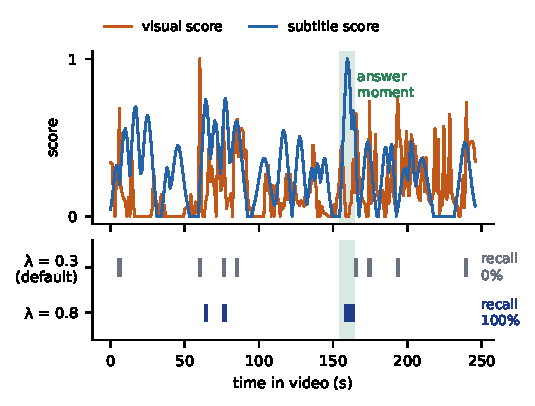
\includegraphics[height=0.6\textheight]{f01_teaser.pdf}
  \par\vspace{1mm}
  \small Question: ``\ldots when the spoon places the meat onto the mashed potatoes and the subtitle mentions `Just pour the\ldots'\,''.\\
  With the default $\lam=0.3$ all 8 frames \bad{miss} the answer moment; with $\lam=0.8$ they \good{hit} it.
\end{frame}

\begin{frame}{Our idea: learn the weight}
  \begin{columns}[T,onlytextwidth]
    \begin{column}{0.5\textwidth}
      \begin{itemize}
        \item Train a \strong{small predictor} that looks at a question and outputs its own $\lam$.
        \item New question types keep appearing, so the predictor learns them \strong{one after another}.
        \item It should learn new types \strong{without forgetting} old ones.
        \item This setting is called \strong{continual learning}.
      \end{itemize}
    \end{column}
    \begin{column}{0.46\textwidth}
      \begin{block}{Four questions we ask}
        \begin{enumerate}
          \item[Q1] Does the best $\lam$ depend on the question type?
          \item[Q2] Can continual learning learn it? Does it forget?
          \item[Q3] If not, what is holding it back?
          \item[Q4] Do better frames give better answers?
        \end{enumerate}
      \end{block}
    \end{column}
  \end{columns}
\end{frame}

% ════════════════════════════════════════════════════════════════════════
\section{Setup}

\begin{frame}{Experimental setup}
  \small
  \begin{columns}[T,onlytextwidth]
    \begin{column}{0.48\textwidth}
      \strong{Data}: LongVideoBench, 753 questions (one per video)\\[1mm]
      \strong{Four question types (tasks)}, learned in order:
      \begin{itemize}
        \item T1 text perception (127) \quad T2 visual perception (237)
        \item T3 text relation (171) \quad\; T4 visual relation (218)
      \end{itemize}
      70\% train / 30\% test; 3 task orders $\times$ 3 seeds = \strong{9 runs}\\[1mm]
      \strong{Predictor}: small 2-layer network, 54 inputs computed from the two score curves
    \end{column}
    \begin{column}{0.48\textwidth}
      \strong{Continual learning methods}: Naive, EWC, LwF, ER (replay), kNN, and Joint (trains on everything, as a reference)\\[1mm]
      \strong{Baselines}:
      \begin{itemize}
        \item default $\lam=0.3$
        \item \textbf{one $\lam$ tuned on the training set}
        \item one $\lam$ per question type
        \item oracle: best $\lam$ for every question (upper limit)
      \end{itemize}
      \strong{Metrics}: recall@8 = share of answer moments hit by the 8 frames; ACC = final average; FM = forgetting
    \end{column}
  \end{columns}
\end{frame}

% ════════════════════════════════════════════════════════════════════════
\section{Q1: Does the Best Weight Depend on the Question?}

\begin{frame}{Q1: types want different weights}
  \centering
  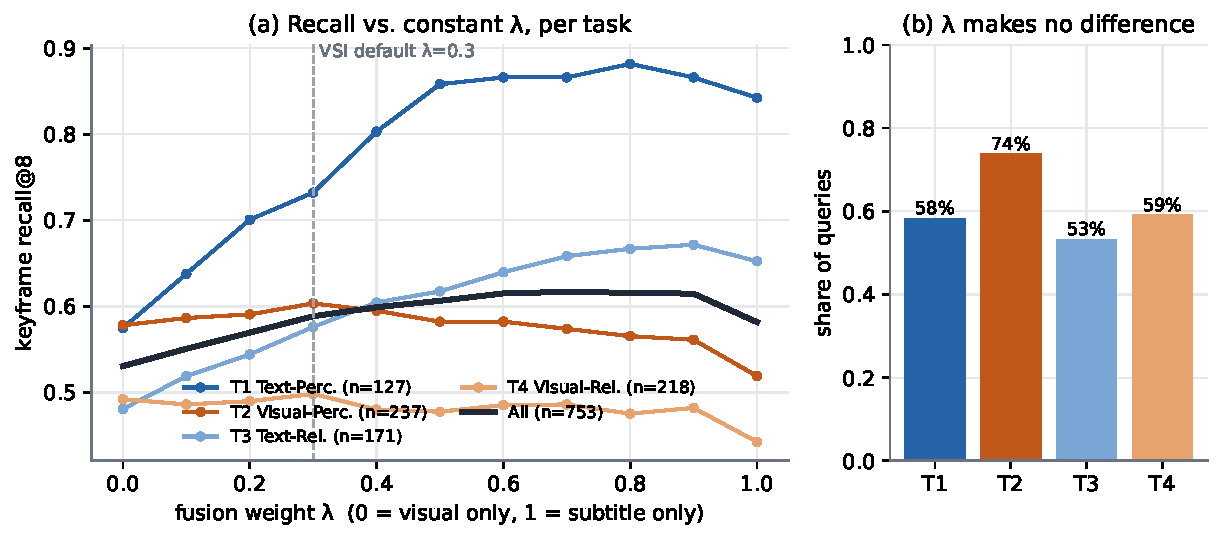
\includegraphics[width=0.82\textwidth]{f02_headroom.pdf}
  \par\vspace{1mm}
  \small Text tasks (blue) peak at $\lam=0.8$--$0.9$; visual tasks (orange) peak at $\lam\le0.3$.\\
  T1: moving $\lam$ from 0.3 to 0.8 raises recall from \strong{0.73 to 0.88}. But \bad{53--74\%} of questions do not react to $\lam$ at all.
\end{frame}

\begin{frame}{Q1: question by question}
  \begin{columns}[c,onlytextwidth]
    \begin{column}{0.58\textwidth}
      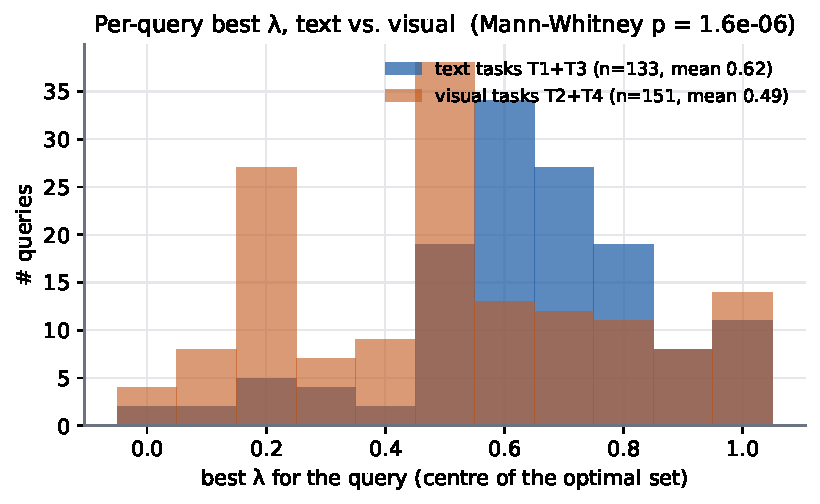
\includegraphics[width=\linewidth]{f03_premise.pdf}
    \end{column}
    \begin{column}{0.38\textwidth}
      Only the 284 questions where $\lam$ matters:
      \begin{itemize}
        \item text questions: mean best $\lam$ = \strong{0.62}
        \item visual questions: mean best $\lam$ = \strong{0.49}
        \item $p = 1.6\times10^{-6}$
      \end{itemize}
      \vspace{2mm}
      \begin{block}{Answer to Q1}
        Yes. The best weight clearly depends on the question type.
      \end{block}
    \end{column}
  \end{columns}
\end{frame}

\begin{frame}{Q1: where is the room to improve?}
  \begin{columns}[c,onlytextwidth]
    \begin{column}{0.58\textwidth}
      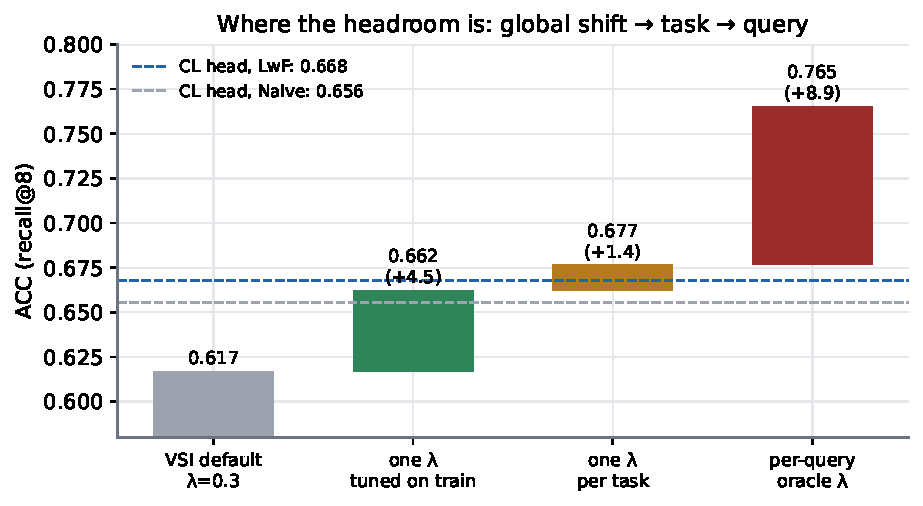
\includegraphics[width=\linewidth]{f16_decomp.pdf}
    \end{column}
    \begin{column}{0.38\textwidth}
      \begin{itemize}
        \item Tune one global $\lam$: \good{+4.5}
        \item One $\lam$ per type: only \strong{+1.4} more
        \item Best $\lam$ per question: \strong{+8.9} more
      \end{itemize}
      \vspace{2mm}
      \begin{alertblock}{Takeaway}
        Most of the gain is in \textbf{per-question} differences, and only a minority of questions carry that signal.
      \end{alertblock}
    \end{column}
  \end{columns}
\end{frame}

% ════════════════════════════════════════════════════════════════════════
\section{Q2 \& Q3: What Does Continual Learning Learn?}

\begin{frame}{Q2: main results (9 runs)}
  \begin{columns}[c,onlytextwidth]
    \begin{column}{0.56\textwidth}
      \centering
      \small
      \begin{tabular}{lccc}
        \toprule
        Method & ACC $\uparrow$ & FM $\downarrow$ & vs.\ tuned \\
        \midrule
        Default $\lam=0.3$ & 0.617 & -- & $-$4.5 \\
        \rowcolor{mbzuai-light-gray}
        One tuned $\lam$ & 0.662 & -- & -- \\
        One $\lam$ per type & 0.677 & -- & +1.4 \\
        Oracle & 0.765 & -- & +10.3 \\
        \midrule
        Naive & 0.656 & 0.029 & $-$0.7 \\
        EWC & 0.662 & 0.023 & $-$0.1 \\
        \rowcolor{mbzuai-light-gray}
        LwF & \textbf{0.668} & \textbf{0.015} & +0.6 \\
        ER & 0.660 & 0.021 & $-$0.3 \\
        Joint (ref.) & \textbf{0.668} & \textbf{0.015} & +0.6 \\
        kNN & 0.645 & 0.005 & $-$1.7 \\
        \bottomrule
      \end{tabular}
    \end{column}
    \begin{column}{0.4\textwidth}
      \begin{itemize}
        \item All methods beat the default by \good{4--5 points}, in \strong{9 of 9} runs.
        \item But compared with \strong{one tuned $\lam$}, the best methods gain only \bad{+0.6}.
        \item None reaches one $\lam$ per type.
        \item LwF and Joint forget about half as much as Naive, but only in 6 of 9 runs.
      \end{itemize}
    \end{column}
  \end{columns}
\end{frame}

\begin{frame}{Q2: run by run}
  \centering
  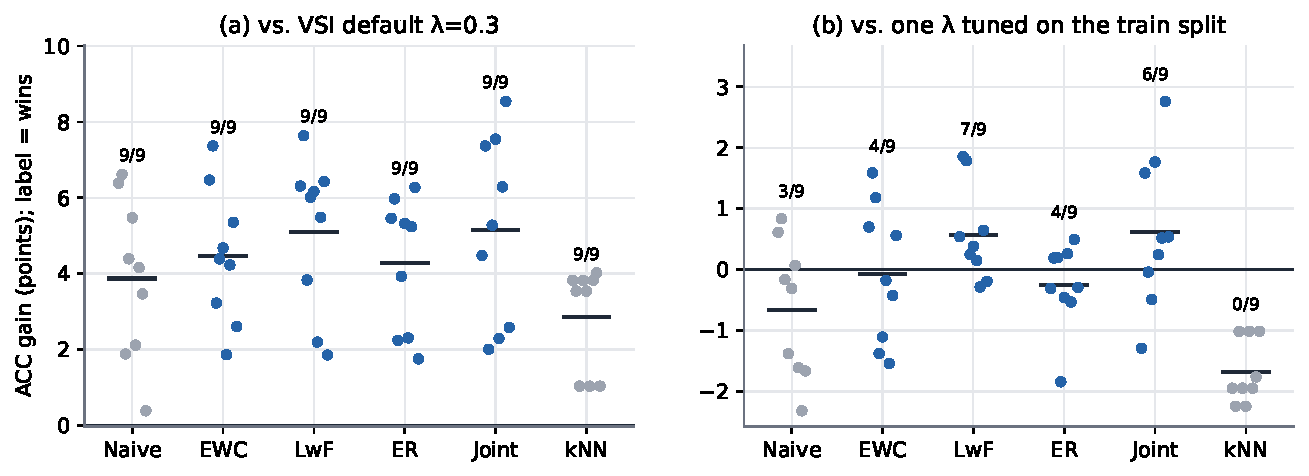
\includegraphics[width=0.88\textwidth]{f10_paired.pdf}
  \par\vspace{1mm}
  \small Each dot is one run. (a) Against the default: always better. (b) Against one tuned $\lam$: \strong{about even}.\\
  Lesson: compare learned weights with a \textbf{tuned} constant, not with the paper's default.
\end{frame}

\begin{frame}{Q3: one weight for every type}
  \centering
  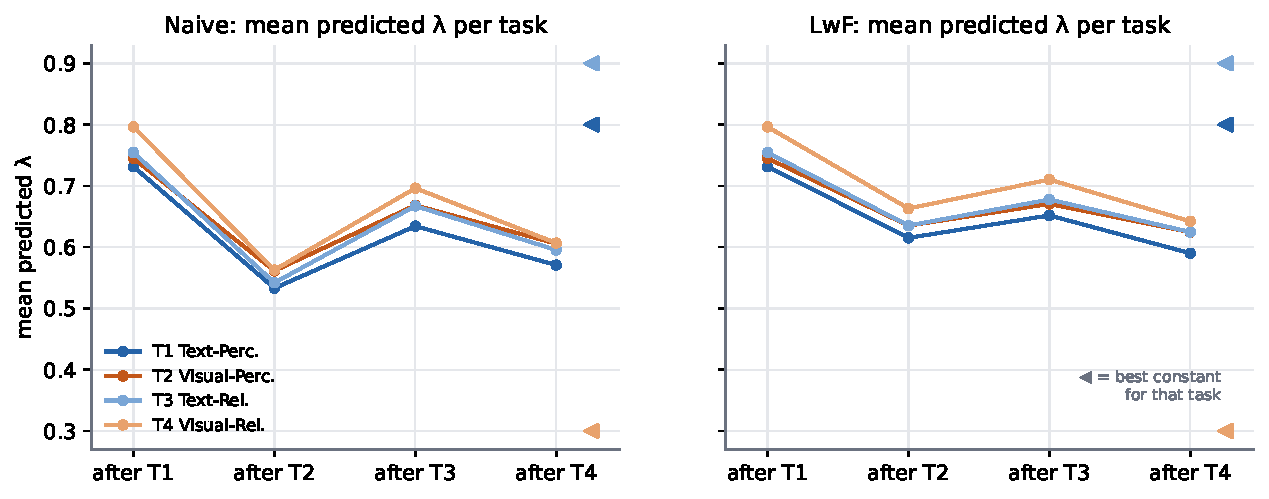
\includegraphics[width=0.86\textwidth]{f12_lambda_rounds.pdf}
  \par\vspace{1mm}
  \small Average predicted $\lam$ for each question type after each training stage. Triangles = best $\lam$ for that type.\\
  The four lines overlap at about 0.6: it learned a \strong{better global value}, not \bad{different values per type}.
\end{frame}

\begin{frame}{Q3: why no differences?}
  \begin{columns}[T,onlytextwidth]
    \begin{column}{0.48\textwidth}
      \begin{block}{1. Sparse training signal}
        62\% of questions give the same result for every $\lam$, so almost all learning comes from the remaining third.
      \end{block}
      \begin{block}{2. No question-type information}
        The inputs only describe the two score curves, which look similar across question types. Adding the question text made it \emph{worse} (overfitting on 753 questions).
      \end{block}
    \end{column}
    \begin{column}{0.48\textwidth}
      \begin{exampleblock}{Why forgetting is small}
        All types end up with similar weights, so learning a new type overwrites little.\\[1mm]
        Still visible: after T2, Naive drops all weights to 0.55; LwF stays steadier.
      \end{exampleblock}
    \end{column}
  \end{columns}
\end{frame}

% ════════════════════════════════════════════════════════════════════════
\section{Q4: Do Better Frames Give Better Answers?}

\begin{frame}{Q4: answering with Qwen3-VL-8B}
  \begin{columns}[c,onlytextwidth]
    \begin{column}{0.48\textwidth}
      \centering
      \small
      \begin{tabular}{lc}
        \toprule
        Frames chosen by & QA accuracy \\
        \midrule
        Even spacing & 0.615 \\
        $\lam=0$ (picture only) & 0.604 \\
        \rowcolor{mbzuai-light-gray}
        $\lam=0.3$ (default) & 0.631 \\
        $\lam=0.7$ (best recall) & 0.627 \\
        $\lam=1$ (subtitles only) & 0.615 \\
        Oracle $\lam$ & 0.649 \\
        \midrule
        LwF predictor$^*$ & +0.4 vs.\ default \\
        \bottomrule
      \end{tabular}
      \par\vspace{1mm}
      {\scriptsize $^*$ paired, on its own test questions; 95\% CI $[-1.5, +2.3]$, not significant}
    \end{column}
    \begin{column}{0.48\textwidth}
      \begin{itemize}
        \item The learned weight and the default give \strong{the same accuracy}.
        \item Even the oracle weight adds only \strong{1.8 points}.
        \item The best-recall weight (0.7) answers slightly \bad{worse} than 0.3.
      \end{itemize}
      \vspace{2mm}
      \begin{alertblock}{So}
        Better recall@8 does not automatically mean better answers.
      \end{alertblock}
    \end{column}
  \end{columns}
\end{frame}

\begin{frame}{Q4: it matters for some questions}
  \centering
  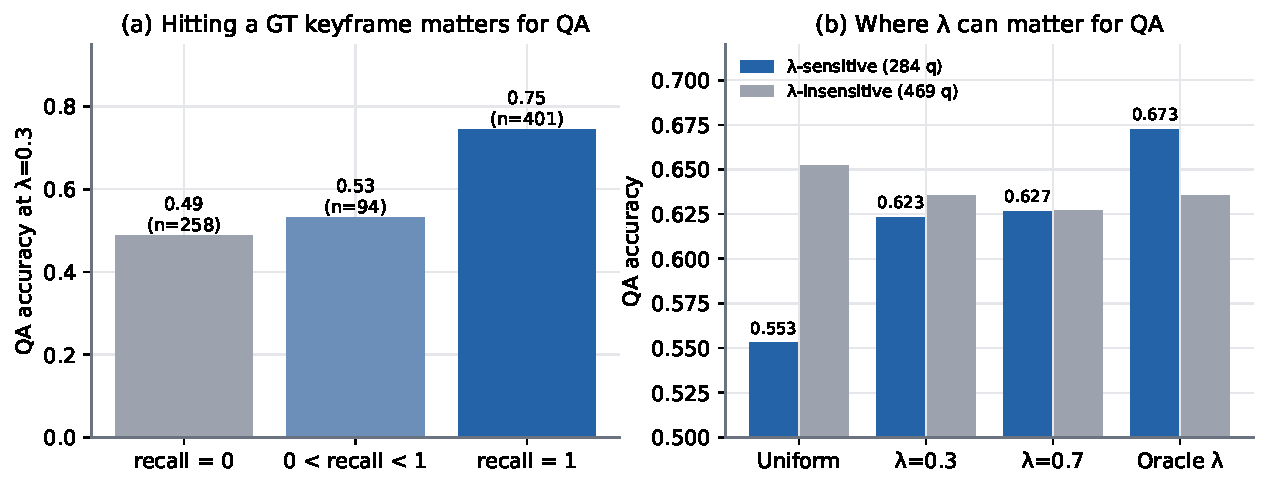
\includegraphics[width=0.84\textwidth]{f15_qa_recall.pdf}
  \par\vspace{1mm}
  \small (a) Hitting the answer moment matters: accuracy \strong{0.49} with no hit vs.\ \strong{0.75} with all hits.\\
  (b) On the 284 questions where $\lam$ changes the frames, the oracle weight answers \good{5 points} more; elsewhere nothing changes.
\end{frame}

% ════════════════════════════════════════════════════════════════════════
\section{Lessons and Conclusion}

\begin{frame}{Four mistakes we fixed}
  \small
  Each one ran without errors but gave wrong results.
  \vspace{2mm}

  \begin{tabular}{p{0.24\textwidth}p{0.68\textwidth}}
    \toprule
    Problem & What happened \\
    \midrule
    Frames vs.\ seconds & Annotations are frame numbers, scores are per second: 94\% of questions got zero recall. \\
    Annotation frame rate & LongVideoBench counts frames at a fixed \strong{24 fps}, not the real 30 fps; annotations were placed too early. \\
    Short videos dropped & Videos $\le$16 s could not fill VSI's 4$\times$4 grid and were silently skipped (197 questions). \\
    Train vs.\ test weight & Trained on the average $\lam$ but tested on the most likely one, which picked $\lam=0$ or $1$: learned weights looked \bad{3--5 points worse} than the default. \\
    \bottomrule
  \end{tabular}
\end{frame}

\begin{frame}{Summary}
  \begin{enumerate}
    \item \strong{The best weight depends on the question type.} Text questions want more subtitle, visual questions more picture.
    \vspace{2mm}
    \item \strong{Continual learning beats the default, but only ties a tuned constant.} The predictor collapses to one weight for all types; forgetting is small.
    \vspace{2mm}
    \item \strong{Better frames help answers only for some questions.} About 38\% of questions react to $\lam$; there the best weight adds 5 points.
    \vspace{2mm}
    \item \strong{Next step:} predict \emph{per-question} differences from sparse signal, e.g., give the predictor the question type, or start from one $\lam$ per type and learn corrections.
  \end{enumerate}
\end{frame}

{
\setbeamertemplate{footline}{}
\setbeamertemplate{frametitle}{}
\begin{frame}[t]
  \mbzuaiThankYou
\end{frame}
}

% ════════════════════════════════════════════════════════════════════════
\appendix
\section*{Backup}

\begin{frame}{Backup: annotation frame rate}
  \centering
  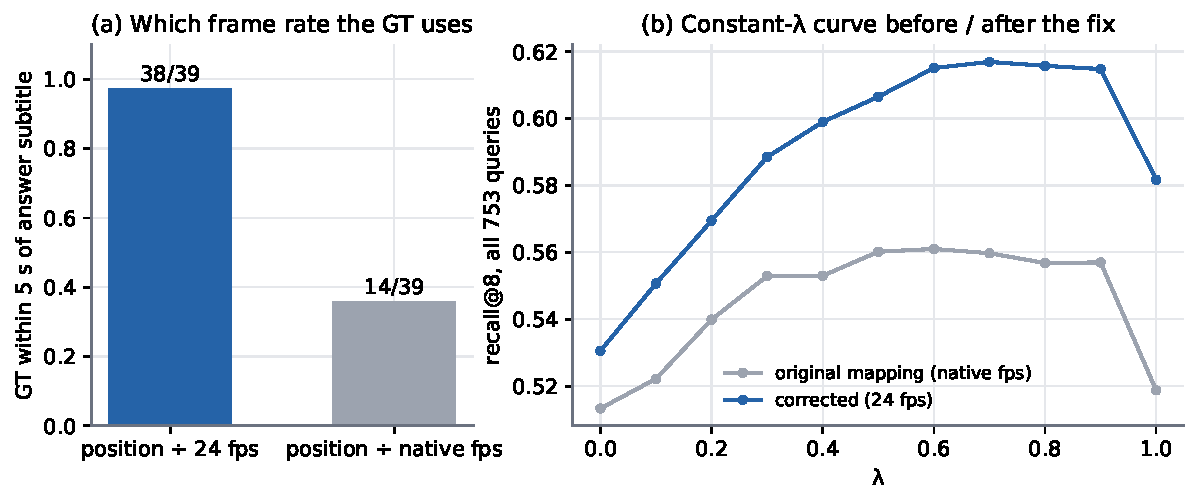
\includegraphics[width=0.85\textwidth]{f08_gtfix.pdf}
  \par\small (a) 38 of 39 annotations match the answer subtitle at 24 fps, only 14 at the real frame rate. (b) Recall vs.\ $\lam$ before and after.
\end{frame}

\begin{frame}{Backup: train/test mismatch}
  \centering
  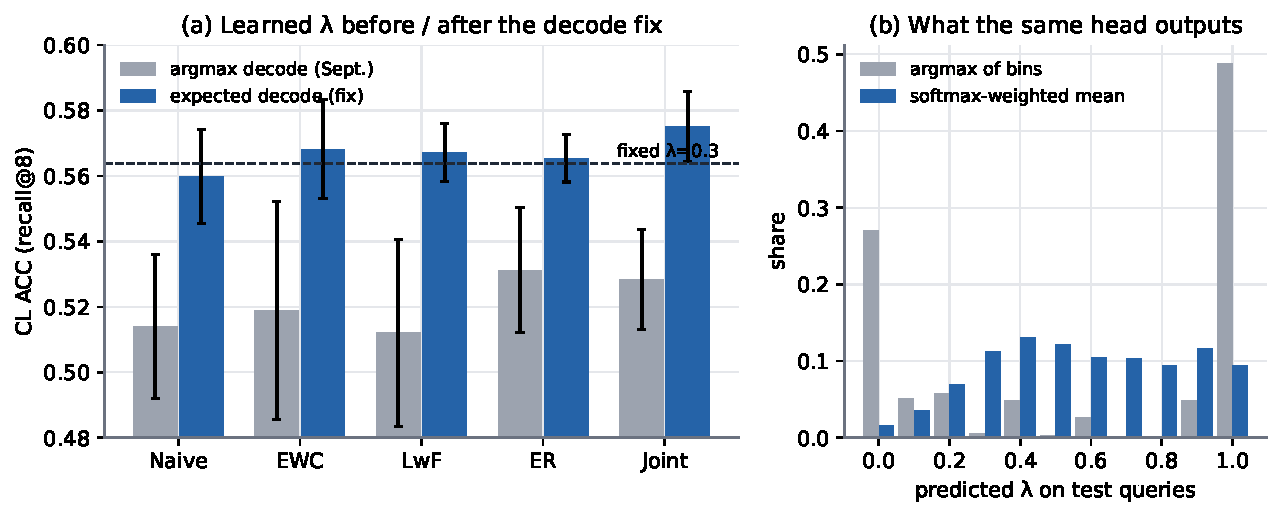
\includegraphics[width=0.85\textwidth]{f05_decode.pdf}
  \par\small (a) Continual learning accuracy before and after the fix (old annotations). (b) The same predictor puts its probability on $\lam=0$ and $\lam=1$.
\end{frame}

\begin{frame}{Backup: predictor inputs}
  \centering
  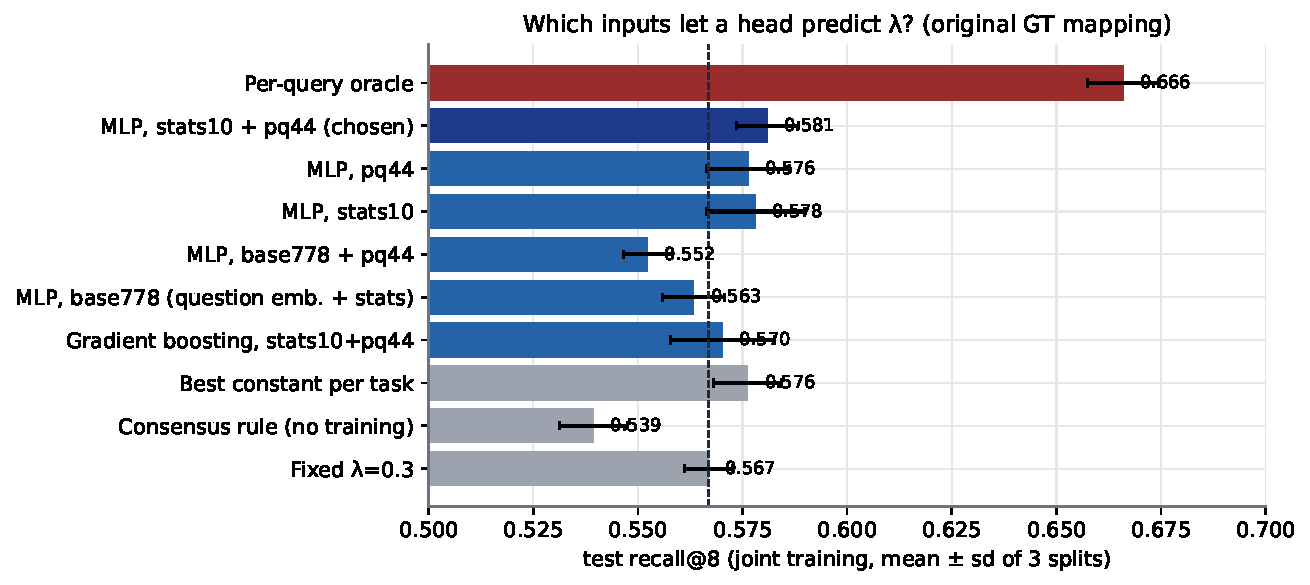
\includegraphics[height=0.72\textheight]{f07_features.pdf}
\end{frame}

\end{document}
